\chapter{Market Analysis}

\section{Industry Overview and Market Potential}

Drones are transforming agriculture by offering innovative solutions to enhance efficiency and sustainability. As reported by \textit{The New York Times} \cite{chaundler2021}, companies like CO2 Revolution are using drones to plant seeds in inaccessible areas, showcasing the potential of drone technology in reforestation and agricultural applications.

The global agricultural sector faces significant challenges, including the need to increase food production to meet the demands of a growing population and to address climate change impacts \citep{nazarov2023}. Traditional farming methods are often insufficient, leading to a surge in the adoption of drones for various agricultural purposes.

\subsection{Applications of Drones in Agriculture}

Drones are used in agriculture for a wide range of applications:

\begin{itemize} 
	\item \textbf{Crop Monitoring and Mapping:} Drones provide high-resolution aerial imagery, enabling farmers to monitor crop health, identify pest infestations, and assess soil conditions in real-time \citep{nazarov2023, alliedmarketresearch2021}. 
	\item \textbf{Precision Spraying:} Equipped with advanced navigation systems, drones can apply fertilizers, pesticides, and herbicides precisely where needed, reducing chemical usage and minimizing environmental impact \citep{guardianagriculture, plantdiseasedetection2023}. 
	\item \textbf{Irrigation Management:} Drones assist in detecting variations in soil moisture levels using thermal sensors, helping optimize irrigation systems and conserve water resources \citep{nazarov2023}. 
	\item \textbf{Planting and Seeding:} Some drones are designed to plant seeds over large areas efficiently, particularly useful in reforestation efforts and hard-to-reach terrains \citep{chaundler2021}. 
\end{itemize}

\subsection{Market Growth and Potential}

The agricultural drone market is experiencing significant growth. Valued at \$0.88 billion in 2020, it is projected to reach \$5.89 billion by 2030, with a compound annual growth rate (CAGR) of 22.4\% \citep{alliedmarketresearch2021}. Key factors contributing to this growth include:

\begin{itemize} 
	\item \textbf{Demand for Increased Food Production:} Global population growth drives the need for higher agricultural output, encouraging the adoption of efficient technologies like drones \citep{nazarov2023}. 
	\item \textbf{Technological Advancements:} Improvements in drone capabilities, such as enhanced sensors and longer flight times, make them more practical for agricultural applications \citep{guardianagriculture}. 
	\item \textbf{Adoption of Precision Farming Techniques:} Farmers are increasingly using drones for site-specific crop management to optimize resource use and increase yields \citep{alliedmarketresearch2021}. 
\end{itemize}

\subsection{Challenges and Opportunities}

While the potential is significant, the adoption of drones in agriculture faces several challenges:

\begin{itemize} 
	\item \textbf{Regulatory Barriers:} Strict government regulations on airspace and drone operations can hinder deployment \citep{nazarov2023}. 
	\item \textbf{High Initial Costs:} The expense of acquiring and maintaining advanced drones may be prohibitive for small-scale farmers \citep{alliedmarketresearch2021}. 
	\item \textbf{Privacy and Safety Concerns:} The use of drones can raise privacy issues and pose safety risks to people and animals if not operated correctly \citep{petiole_drones_risks}. 
\end{itemize}

Opportunities to address these challenges include:

\begin{itemize} 
	\item \textbf{Government Support:} Initiatives like Austria's "Smart Farming" action plan aim to integrate digital technologies into agriculture, providing funding and resources to farmers \citep{smartfarming2023}. 
	\item \textbf{Technological Innovations:} Developing user-friendly and cost-effective drones can lower barriers to entry \citep{guardianagriculture}. 
	\item \textbf{Privacy and Safety Enhancements:} Implementing measures such as geofencing and privacy-by-design is vital for mitigating privacy and safety concerns. Geofencing restricts drones from flying in specific, predefined areas, such as residential neighborhoods or around sensitive infrastructure, helping to prevent unwanted intrusions and ensure responsible drone use. Privacy-by-design involves minimizing data collection, securing collected data, and ensuring transparency, which collectively enhance trust and compliance with privacy regulations \citep{secure_redact_drones_privacy}. 
\end{itemize}

\section{Target Group Definition}

Our ideal customers are small to medium-sized agricultural enterprises, individual farmers, and agricultural cooperatives who have limited budgets compared to large enterprises. They are seeking cost-effective solutions to modernize their farming operations with drone technology without the high expenses associated with advanced onboard systems.

\textbf{Key Characteristics}

\begin{itemize}
	\item \textbf{Demographics}: Decision-makers aged 35--60 with practical experience in agriculture, often fitting the 'Pragmatic Traditionals' or 'Adaptive Pragmatic Middle' Sinus-Milieus \cite{sinus_institut_2024}. 
	\item \textbf{Geographics}: Located in rural agricultural regions such as Lower Austria, Styria, Upper Austria, and Tyrol. 
	\item \textbf{Psychographics}: Value efficiency, sustainability, and are open to adopting new technologies that improve their farming practices. 
	\item \textbf{Behavioral}: Make purchase decisions based on cost-benefit analysis, attend local agricultural events, rely on recommendations from peers and local networks. 
	\item \textbf{Needs}: Affordable and reliable drone tracking systems that are easy to implement and help optimize farming operations. 
	\item \textbf{Technographics}: Moderate technological proficiency, use basic agricultural management tools, interested in user-friendly technology solutions. 
\end{itemize}

\section{Buyer Personas}

\textbf{Persona 1: Thomas Bauer}

\begin{itemize}
	\item \textbf{Age}: 52 
	\item \textbf{Role}: Owner of a medium-sized family farm 
	\item \textbf{Location}: Lower Austria
	\item \textbf{Goals}: Increase crop yields and operational efficiency through affordable technology 
	\item \textbf{Pain Points}: Limited budget for high-end drones; needs cost-effective tracking solutions without extensive technical expertise 
	\item \textbf{Behavior}: Reads local agricultural journals, attends regional farming expos, values practical and easy-to-use solutions 
\end{itemize}

\textbf{Persona 2: Maria Hofer}

\begin{itemize} 
	\item \textbf{Age}: 40 
	\item \textbf{Role}: Owner of a small organic farm 
	\item \textbf{Location}: Graz, Styria 
	\item \textbf{Goals}: Implement sustainable farming practices with the help of affordable technology 
	\item \textbf{Pain Points}: Needs reliable tracking solutions that align with organic farming principles; constrained by a tight budget 
	\item \textbf{Behavior}: Active in local farming communities, follows agricultural trends online, seeks eco-friendly and cost-effective solutions 
\end{itemize}

\textbf{Persona 3: Andreas Schneider}

\begin{itemize} 
	\item \textbf{Age}: 55 
	\item \textbf{Role}: Manager of a farming cooperative 
	\item \textbf{Location}: Upper Austria 
	\item \textbf{Goals}: Enhance productivity for cooperative members through shared resources and technology 
	\item \textbf{Pain Points}: Finding affordable technology solutions that can be easily adopted by multiple farmers with varying levels of technical skill 
	\item \textbf{Behavior}: Engages with cooperative members, attends agricultural seminars, values solutions that offer collective benefits 
\end{itemize}

\section{Competitor Analysis}

The agricultural drone market is increasingly competitive in Austria and globally, with key players offering advanced solutions for precision farming. This analysis focuses on three major competitors relevant to the Austrian market:

\begin{enumerate} 
	\item \textbf{Dronetech (Austria):} An Austrian drone service provider, Dronetech has partnered with Huawei to develop 5G-enabled drone solutions for smart farming. They modify DJI drones with custom 3D-printed parts to optimize them for specific agricultural needs \cite{dronetech_instagram, dji_m300}. Equipped with additional high-resolution cameras and sensors, these drones use Huawei's cloud computing and AI for real-time data analysis. This allows for precise application of water, fertilizers, and pesticides, significantly reducing waste and environmental impact. A key challenge they face is the current network coverage limitations for 5G-enabled drones \cite{huawei_dronetech_2022, huawei_boosting_farming_2022, dronetech_smart_farming_project}.

	\item \textbf{DJI (China):} A global leader in drone technology, DJI Agriculture offers expensive high-tech drones such as the DJI Agras T50, T25, and Mavic 3M, designed for agricultural tasks like spraying, mapping, and crop monitoring. These drones utilize RTK/GNSS for precise positioning, phased-array radar and vision sensors for obstacle avoidance, and Radio, WiFi, and Bluetooth for communication \cite{dji_ag_t25, dji_ag_t50}. They also offer accessories such as the DJI Relay to enhance communication in complex environments. In Austria, DJI's agricultural products are distributed through partners like Drohnenring, providing consultation, sales, training, and support services \cite{drohnenring_2024, dji_agriculture_2024}.
	
	\item \textbf{AgEagle (USA):} AgEagle Aerial Systems Inc. specializes in agricultural mapping solutions, offering drones like the eBee X and multispectral sensors such as RedEdge-P and Altum-PT. These drones are equipped with RTK and GNSS for precise positioning, delivering centimeter-level accuracy without the need for ground control points. Communication is ensured through radio links with a range of up to 3 km and secure encryption. For safe and efficient flight, the drones utilize LiDAR sensors for obstacle avoidance and controlled landings. Additionally, AgEagle supports their hardware with software tools like eMotion and Measure Ground Control for streamlined flight planning and data processing \cite{ageagle_agriculture_2024, ageagle_agriculture_ebee}.
\end{enumerate}

\subsection{Competitive Landscape}

The agricultural drone market in Austria features both local companies like Dronetech, leveraging partnerships with global tech firms to offer innovative solutions, and international players like DJI and AgEagle, providing advanced drone technology and comprehensive agricultural services. Competition centers on integrating cutting-edge technologies such as 5G connectivity, AI, RTK/GNSS positioning, and multispectral imaging to enhance precision farming practices. Each competitor offers sophisticated communication systems, precise positioning capabilities, and advanced software solutions to meet the evolving needs of modern agriculture.

\subsection{Our Differentiation and Positioning}

Our ground-based 3D drone tracking system distinguishes itself by offering an affordable and accessible solution that eliminates the need for expensive onboard positioning and obstacle avoidance systems. By utilizing ground-based 3D tracking through calibrated and synchronized stations with advanced image processing, our system allows for the deployment of simpler drones without sophisticated onboard equipment.

This approach provides several key benefits:

\begin{itemize} 
	\item \textbf{Enhanced Drone Efficiency and Cost Savings:} By removing heavy onboard sensors and communication equipment, drones become lighter and consume less energy, resulting in increased flight times and the ability to cover larger areas per mission. This also allows drones to carry additional payloads such as seeds, fertilizers, or pesticides, enhancing operational efficiency in tasks like seed planting or crop spraying. The reduction in onboard complexity lowers maintenance requirements and decreases the risk of technical failures, ensuring consistent operational capability. Overall, this leads to significant cost savings, making precision agriculture technologies more accessible to farmers with limited budgets.
	
	\item \textbf{Secure and Independent Communication System:} Operating within a local, enclosed communication system independent of network infrastructure ensures reliable performance regardless of connectivity issues common in rural agricultural areas. Unlike competitors relying on 5G networks, our system does not depend on external networks, enhancing operational reliability and improving data security and privacy. Processing tracking data locally reduces reliance on cloud services, giving farmers greater control over their data without concerns about transmitting sensitive information over public networks.
	
	\item \textbf{Scalability and Flexibility:} Our ground stations can track multiple drones simultaneously without adding complexity or weight to the drones themselves. This allows for scalable operations, enabling large-scale agricultural tasks to be performed efficiently. Farmers can easily expand their drone fleets without significant additional investment in drones with expensive onboard equipment.
	
	\item \textbf{Integrated Software Solutions:} While our system reduces the need for onboard software, we provide user-friendly ground-based software for flight planning, real-time monitoring, and data analysis. Our software integrates with the ground stations to offer seamless control and management of drone operations, tailored to the specific needs of the agricultural sector (theoretical as building the drone is not part of this diploma thesis).
\end{itemize}

We position ourselves as a provider of innovative, cost-effective drone tracking solutions tailored to Austria's agricultural sector. Our ground-based system addresses challenges like network coverage limitations, high equipment costs, and drone payload restrictions, making it more accessible for small to medium enterprises. By removing the need for expensive onboard systems and reducing maintenance complexities, we offer a practical, efficient tool that improves farming operations without requiring substantial investment. This unique value proposition allows farmers to adopt modern drone technology, enhancing their efficiency and sustainability at a lower cost.

\begin{figure}
	[H] 
	\centering 
	\hspace*{-1.5cm} 
	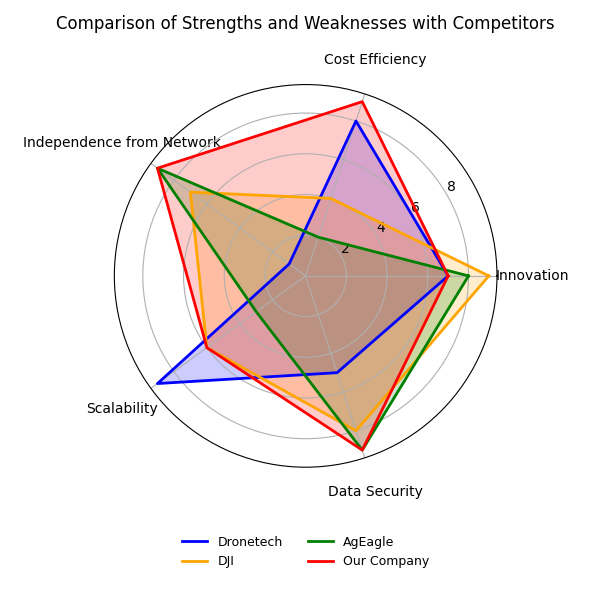
\includegraphics[width=400pt]{figures/competitors.png} 
	\caption{Strengths and Weaknesses of Agricultural Drone Competitors} 
	\label{image} 
\end{figure}

\section{Conclusion}

The market analysis reveals a significant opportunity for our ground-based 3D drone tracking system in the agricultural sector. As drone adoption in agriculture accelerates, our solution addresses key challenges like high costs, dependence on network infrastructure, and the complexity of onboard systems by eliminating the need for expensive onboard communication, positioning, and obstacle avoidance equipment. By enabling the use of simpler, more affordable drones with increased payload capacity and simplified maintenance, we offer a unique value proposition that differentiates us from competitors relying on complex onboard technologies. Our system aligns with the needs of small to medium agricultural enterprises seeking efficient and sustainable technologies without the barriers of high initial investment and technical complexity. Further research and engagement with industry stakeholders will refine our understanding of target customers and support a successful market entry, positioning us as a competitive player in the agricultural drone market focused on accessibility and practicality.